\section{第二组公理:顺序公理}
本组公理规定了“介于”(或“在……之间”)这个概念.
根据这个概念,直线上的、平面上的和空间中的点才有顺序可言.
\begin{axiom}[顺序公理I]\label{axiom:欧氏几何.顺序公理1}
在一直线上的点有一定的相互关系.
我们特别用“介于”(或“在……之间”)来描述它.
\begin{enumerate}
	\item 若一点\(B\)在一点\(A\)和一点\(C\)之间
	(如\cref{figure:欧氏几何.直线上点的顺序1}),
	则\(A\)、\(B\)和\(C\)是一直线上的不同的三点,
	同时\(B\)也在\(C\)和\(A\)之间.
	\begin{figure}[htb]
		\centering
		
\begin{tikzpicture}
			\draw[fill=black] (0,0)--(1,0)node[above]{\(A\)}circle(1pt)
			--(1.7,0)node[above]{\(B\)}circle(1pt)
			--(3,0)node[above]{\(C\)}circle(1pt)
			--(4,0);
		\end{tikzpicture}
		\caption{直线上点的顺序}
		\label{figure:欧氏几何.直线上点的顺序1}
	\end{figure}

	\item 对于两点\(A\)和\(B\)(如\cref{figure:欧氏几何.直线上点的顺序2}),
	直线\(AB\)上恒至少有一点\(C\),使得\(B\)在\(A\)和\(C\)之间.
	\begin{figure}[htb]
		\centering
		
\begin{tikzpicture}
			\draw[fill=black] (0,0)--(1,0)node[above]{\(A\)}circle(1pt)
			--(2.4,0)node[above]{\(B\)}circle(1pt)
			--(3,0)node[above]{\(C\)}circle(1pt)
			--(4,0);
		\end{tikzpicture}
		\caption{直线上点的顺序}
		\label{figure:欧氏几何.直线上点的顺序2}
	\end{figure}

	\item 一直线的任意三点中,至多有一点在其他两点之间.
\end{enumerate}
\end{axiom}

在上述三条{\bf 直线顺序公理}之外,还需要一条{\bf 平面顺序公理}.

\begin{axiom}[顺序公理II]\label{axiom:欧氏几何.顺序公理2}
考虑一直线\(l\)上的两点\(A\)和\(B\).
我们把这一对点\(A\)和\(B\)确定的介于它们的点的集合叫做一条\DefineConcept{线段},记作\(AB\)(或\(BA\)).
在\(A\)和\(B\)之间的点叫做线段\(AB\)的点,或线段\(AB\)的\DefineConcept{内点};
\(A\)和\(B\)叫做线段\(AB\)的\DefineConcept{端点};
直线\(l\)上的其他点叫做线段\(AB\)的\DefineConcept{外点}.
\begin{enumerate}
	\setcounter{enumi}{3}
	\item 设\(A\)、\(B\)和\(C\)是不在同一直线上的三点,
	\(l\)是平面\(ABC\)上的一直线,
	但\(l\)不通过\(A,B,C\)这三点中的任一点
	(如\cref{figure:欧氏几何.平面上点的顺序1}),
	若直线\(l\)通过线段\(AB\)的一点,则它必定也通过线段\(AC\)或线段\(BC\)的一点.
	\begin{figure}[htb]
		\centering
		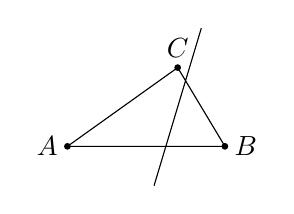
\begin{tikzpicture}
			\draw[fill=black] (-1,0)node[left]{\(A\)}circle(1pt)
			--(1,0)node[right]{\(B\)}circle(1pt)
			--(.4,1)node[above]{\(C\)}circle(1pt)--(-1,0)
			(.1,-.5)--(.7,1.5);
		\end{tikzpicture}
		\caption{平面上点的顺序}
		\label{figure:欧氏几何.平面上点的顺序1}
	\end{figure}
\end{enumerate}
\end{axiom}
直观地说,\cref{axiom:欧氏几何.顺序公理2} 说的就是:
若一直线“冲进”一个三角形的内部,它必定还要再“冲出”这个三角形.
易证:与线段\(AB\)相交的直线\(l\)不同时和\(AC,BC\)这两条线段都相交.
